\begin{figure}[htbp]
\centering
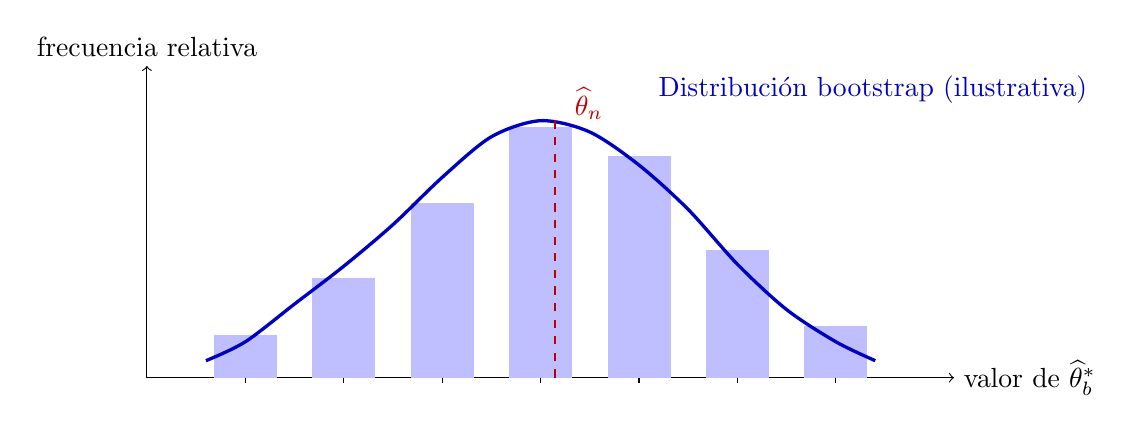
\begin{tikzpicture}[x=1.25cm,y=1.2cm]
  \draw[->] (0,0) -- (8.2,0) node[right] {valor de $\widehat\theta_b^*$};
  \draw[->] (0,0) -- (0,3.3) node[above] {frecuencia relativa};
  \foreach \x in {1,...,7}
    \draw (\x,0) -- (\x,-0.06);
  \foreach \x/\h in {1/0.45,2/1.05,3/1.85,4/2.65,5/2.35,6/1.35,7/0.55}
    \fill[blue!25] (\x-0.32,0) rectangle (\x+0.32,\h);
  \draw[very thick,blue!75!black] plot[smooth] coordinates {
    (0.6,0.18) (1,0.38) (1.5,0.78) (2,1.18) (2.5,1.62)
    (3,2.12) (3.5,2.55) (4,2.72) (4.5,2.60) (5,2.25)
    (5.5,1.78) (6,1.20) (6.5,0.72) (7,0.38) (7.4,0.18)
  };
  \draw[dashed,red!75!black,thick] (4.15,0) -- (4.15,2.8);
  \node[anchor=west,red!75!black] at (4.25,2.9) {$\widehat\theta_n$};
  \node[anchor=west,blue!75!black] at (5.1,3.05) {Distribución bootstrap (ilustrativa)};
\end{tikzpicture}
\caption{Distribución bootstrap ilustrativa de las estimaciones $\widehat\theta_b^*$. Su dispersión describe la variabilidad del estimador bajo remuestreo; la línea roja marca la estimación obtenida con la muestra original.}
\label{fig:distribucion-bootstrap}
\end{figure}